
\documentclass[fleqn,addpoints]{exam}

\usepackage{graphicx}
\usepackage{booktabs}
\usepackage{float}
\usepackage{amsmath}
\usepackage{cancel}
\usepackage{polynom}
\usepackage{caption}
\usepackage{mdwlist}

\newcommand{\degree}{\ensuremath{^\circ}} 

\printanswers

\ifprintanswers 
\usepackage{2in1, lscape} 
\fi

\title{Math 115 \\ Homework 24}
\date{May 24, 2011}

\begin{document}

\maketitle

% \begin{figure}[H]
%   \centering
%   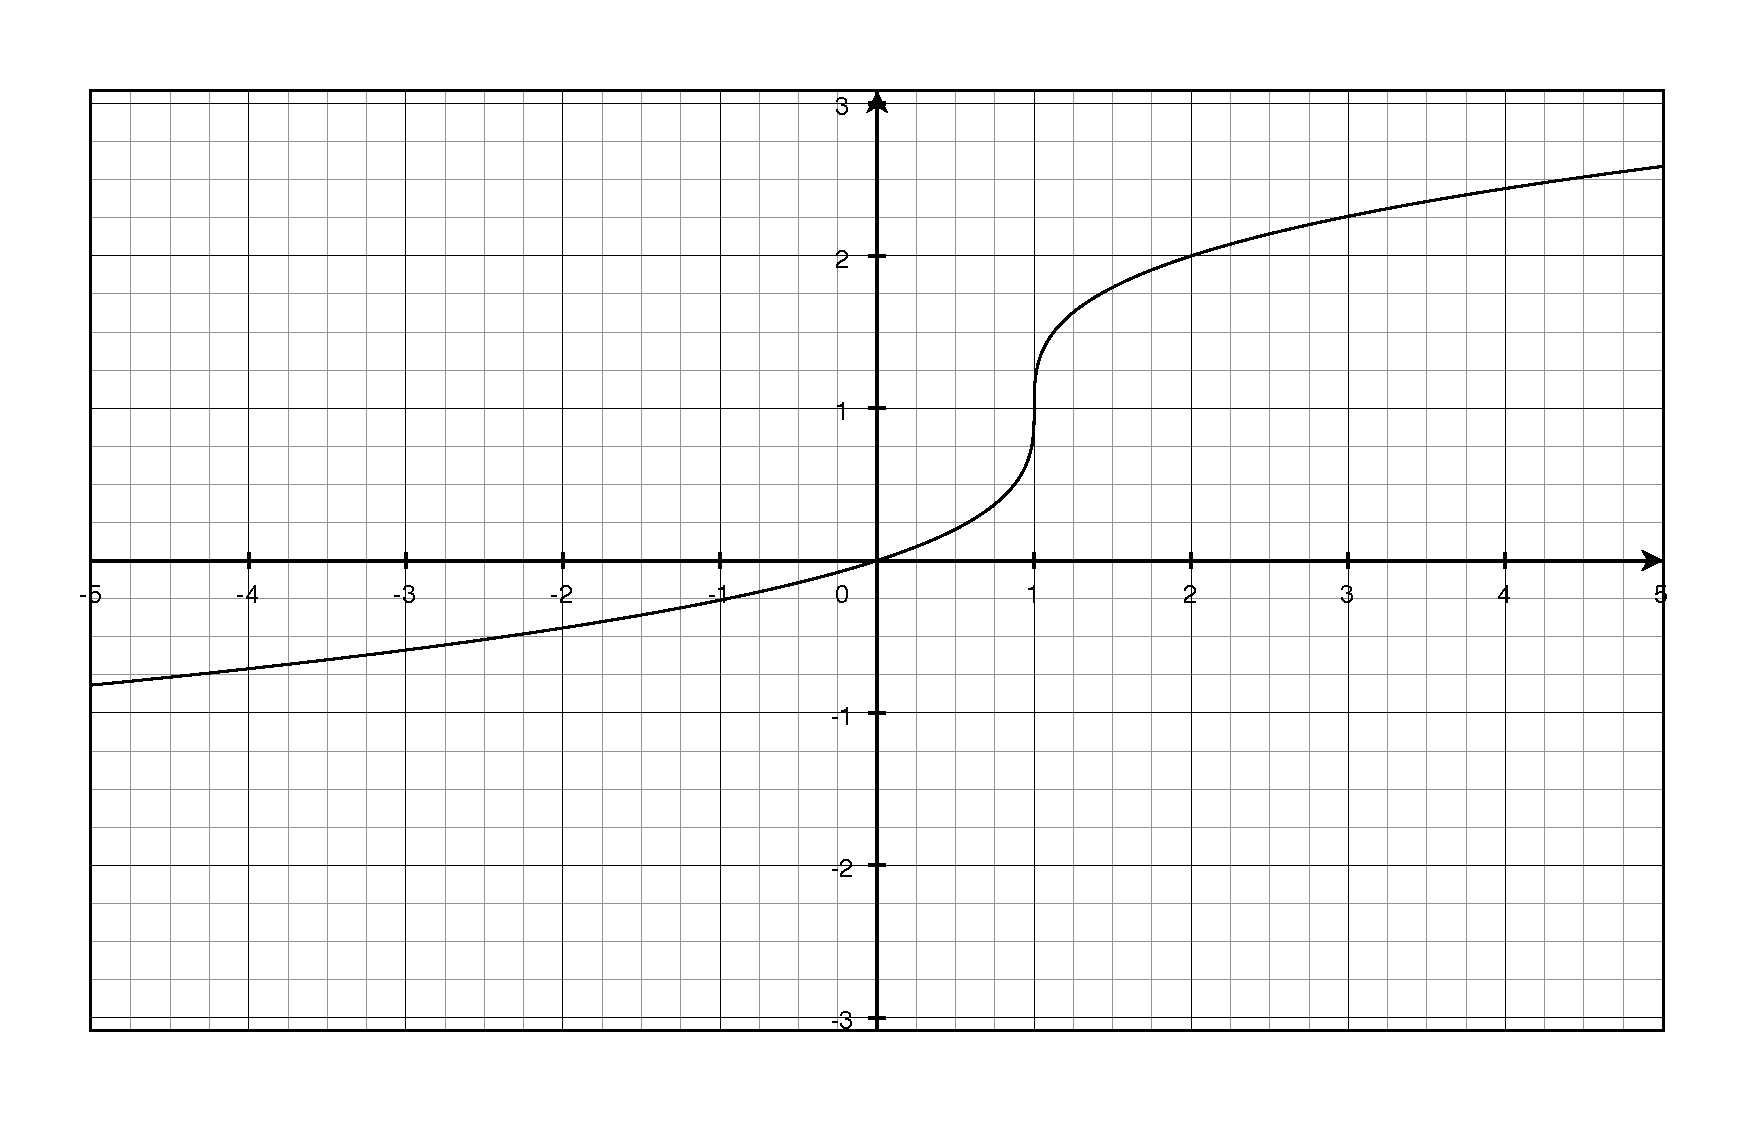
\includegraphics[scale=.3]{question7.eps}
%   \caption*{Question 7}
% \end{figure}

% \begin{tabular}{cc}
% \toprule
% period & amplitude \\
% \midrule
%   $\pi$ & $2$ \\
% \bottomrule
% \end{tabular}

% \ifprintanswers
% \else

\section{Homework}
\begin{itemize*}
  \item pp. 447-449: 1-2, 15-20, 31-35, 46-50, 52-53, 61-62, 91-92
  \item pp. 455-456: 4-5, 10-14, 20-24, 29-30, 43-44, 66-69
\end{itemize*}

% \fi

\section{Extra Credit}
p. 455, questions 35 and 36

\begin{description}
\item[35]
\[
  \frac{\sin x \cos y + \cos x \sin y}{\cos x \cos y - \sin x \sin y} 
    \cdot \frac{1/\cos x \cos y}{1/\cos x \cos y} = \frac{\tan x + \tan y}{1 - \tan x \tan y}
\]

\item[36]
\[
  \frac{\tan x + \tan y}{1 - \tan x \tan y} \cdot \frac{\cot x \cot y}{\cot x \cot y}
    = \frac{\cot x + \cot y}{\cot x \cot y - 1}
\]

\end{description}

\ifprintanswers
\section{Pages 447-449}

\begin{description}

\item[1] 
The angle is in quadrant II because of the signs of the values provided.

\begin{align*}
  \tan x &= \frac{\sqrt{3}}{2} \cdot \left( - \frac{1}{2} \right) = - \sqrt{3} \\
  \cot x &= -\frac{\sqrt{3}}{3} \\ 
  \csc x &= \frac{2 \sqrt{3}}{3} \\
  \sec x &= -2 \\
\end{align*}

\item[2] 
The angle is in quadrant IV because of the signs of the values provided.

\begin{align*}
  \cot x &= \sqrt{3} \\
  \sec x &= -2 \sqrt{3} \\
  \sin x &= - \sqrt{1 - \frac{3}{4}} = -\frac{1}{2} \\
  \csc x &= -2 \\
\end{align*}

\item[15]
d

\[
  \frac{1}{\cos x} \cdot \cos x = 1
\]

\item[16]
a

\[
  \tan x \cdot \csc x = \tan x \frac{1}{\sin x} = \frac{\sin x}{\cos x} \cdot \frac{1}{\sin x} = \sec x
\]

\item[17]
b

\[
  \cot^2 x - \csc^2 x = cot^2 x - (\cot^2 x + 1) = -1
\]

\item[18]
f

\[
  (1 - \cos^2 x)(\csc x) =   (\sin^2 x) \left( \frac{1}{\sin x} \right) = \sin x
\]

\item[19]
e

\[
  \frac{\sin (-x)}{\cos (-x)} = - \frac{\sin x}{\cos x} = - \tan x
\]

\item[20]
c

\[
  \frac{\sin (\pi/2 - x)}{\cos (\pi/2 -x)} = \frac{\cos x}{\sin x} = \cot x
\]

\item[31]
\[
  \frac{\cot x}{\csc x} = \frac{\cos x}{\sin x} \cdot \sin x = \cos x
\]

\item[32]
\[
  \frac{\csc \theta}{\sec \theta} = \frac{\cos \theta}{\sin \theta} = \cot \theta
\]

\item[33]
\[
  \frac{1 - \sin^2 x}{\csc^2 x - 1} = \frac{\cos^2 x}{\cot^2 x} = \sin^2 x
\]

\item[34]
\[
  \frac{1}{\tan^2 x +1} =   \frac{1}{\sec^2} = \cos^2 x
\]

\item[35]
\[
  \sec \alpha \cdot \frac{\sin \alpha}{\tan \alpha} = \frac{\sin \alpha}{\cos \alpha} \cdot \cot \alpha 
    = \tan \alpha \cdot \cot \alpha = 1
\]

\item[46]
\begin{align*}
  \sin^2 x \csc^2 x - \sin^2 x &= \sin^2 x (\csc^2 x - 1)  \\
  &= \sin^2 x \cot^2 x \\
  &= \sin^2 x \cdot \frac{\cos^2 x}{\sin^2 x} \\
  &= \cos^2 x
\end{align*}


\item[47]
\[
  \sin^2 x \sec^2 x - \sin^2 x =   \sin^2 x (\sec^2 x - 1)  = \sin^2 x \cdot \tan^2 x 
\]

\item[48]
\[
  \cos^2 x + \cos^2 x \tan^2 x = \cos^2 x (1 + \tan^2 x) =  \cos^2 x \sec^2 x = 1
\]

\item[49]
\[
  \frac{\sec^2 x - 1}{\sec x - 1} =   \frac{(\sec x - 1)(\sec x + 1)}{\sec x - 1} = \sec x + 1
\]

\item[50]
\[
  \frac{\cos^2 x - 4}{\cos x - 2} =   \frac{(\cos x - 2)(\cos x + 2)}{\cos x - 2} = \cos x + 2
\]

\item[52]
\[
  \cos^4 x - 2 \cos^2 x + 1 = (\cos^2 x - 1)^2 = (\sin^2 x)^2 = \sin^4 x
\]

\item[53]
\[
  \sin^4x - \cos^4 x = (sin^2 x + cos^2 x) (sin^2 x - cos^2 x) = sin^2 x - \cos^2 x
\]

\item[61]
\begin{align*}
  \frac{1}{1 + \cos x} +   \frac{1}{1 - \cos x} &= \frac{1 - \cos x + 1 + \cos x}{1 - \cos^2 x} \\
  &= \frac{2}{\sin^2 x} \\
  &= 2 \csc^2 x
\end{align*}


\item[62]
\begin{align*}
  \frac{1}{\sec x + 1} - \frac{1}{\sec x - 1} &= \frac{\sec x - 1 - \sec x - 1}{\sec^2 x - 1} \\
  &= - \frac{2}{\tan^2 x} \\
  &= - 2 \cot^2 x
\end{align*}

\item[91]
\[
  \ln |\cos x| - \ln|\sin| = \ln|\cot x|
\]

\item[92]
\[
  \ln |\sec x| + \ln|\sin| = \ln|\tan x|
\]

\section{Pages 455-456}
\item[4]
\[
  (\cot^2 y) (\sec^2 y - 1 ) = \cot^2 y \cdot \tan^2 y = 1
\]

\item[5]
\[
  \cos^2 \beta - \sin^2 \beta = 1 - \sin^2 \beta - \sin^2 \beta = 1 - 2 \sin^2 \beta
\]

\item[10]
\begin{align*}
  \cos x + \sin x \tan x &= \cos x + \frac{\sin^2 x}{\cos x} \\
  &= \frac{\cos^2 x + \sin^2 x}{\cos x} \\
  &= \frac{1}{\cos x} = \sec x \\
\end{align*}

\item[11]
\[
  \frac{\csc^2 \theta}{\cot \theta} = \frac{\sin \theta}{\sin^2 \theta \cos \theta} = \frac{1}{\sin \theta \cos \theta} 
    = \sec \theta \csc \theta
\]

\item[12]
\[
  \frac{\cot^3 t}{\csc t} = \frac{\cos^3 t \sin t}{\sin^3 t} = \cos t \cot^2 t = \cos t(\csc^2 t - 1)
\]

\item[13]
\begin{align*}
  \frac{\cot^2 t}{\csc t} &= \frac{\cos^2 t \sin t}{\sin^2 t} \\
  &= \sin t \cot^2 t \\
  &= \sin t(\csc^2 t - 1) \\
  &= \sin t (\frac{1}{\sin t^2 t} - 1) \\
  &= \csc t - \sin t
\end{align*}

\item[14]
\[
  \frac{1}{\tan \beta} + \tan \beta = \frac{1 + \tan^2 \beta}{\tan \beta} = \frac{\sec^2 \beta}{\tan \beta}
\]

\item[20]
\begin{align*}
  \sec x - \cos x &= \frac{1}{\cos x} - \cos x \\
  &= \frac{1 - \cos^2 x}{\cos x} \\
  &= \frac{\sin^2 x}{\cos x} \\
  &= \sin x \tan x
\end{align*}

\item[21]
\begin{align*}
  \sin x \cos x + \sin^3 x \sec x &= \sin x ( \cos x + \frac{\sin^2 x}{\cos x}) \\
  &= \sin x \left( \frac{\cos^2 x \sin^2 x}{\cos x} \right) \\
  &= \tan x \\
\end{align*}

\item[22]
\begin{align*}
  \frac{\sec x + \tan x}{\sec x - \tan x} &= \frac{\sec x + \tan x}{\sec x - \tan x} \cdot \frac{\sec x + \tan x}{\sec x + \tan x} \\
  &= \frac{(\sec x + \tan x)^2}{\sec^2 x - \tan^2 x} \\
  &= \frac{(\sec x + \tan x)^2}{1 + \tan^2 x - \tan^2 x} \\
  &= \sec x + \tan x)^2 \\
\end{align*}

\item[23]
\[
  \frac{1}{\tan x} + \frac{1}{\cot x} = \frac{\cot x + \tan x}{\tan x \cot x} = \tan x + \cot x
\]

\item[24]
\[
  \frac{1}{\sin x} - \frac{1}{\csc x} = \frac{\csc x - \sin x}{\sin x \csc x} = \csc x - \sin x
\]

\item[29]
\[
  \tan \left( \frac{\pi}{2} - \theta \right) \tan \theta = \cot \theta \tan \theta = 1
\]

\item[30]
\[
  \frac{cos[\pi/2 - x]}{\sin[\pi/2 - x]} = \frac{\sin x}{\cos x} = \tan x
\]

\item[43]
\[
  \sin t \csc \left( \frac{\pi}{2} - t \right) = \sin t \sec t = \frac{\sin t}{\cos t} = \tan t
\]

\item[44]
\[
  \sec^2 \left( \frac{\pi}{2} - x \right) - 1 = \csc^2 x - 1 = \cot^2 x
\]

\item[66]
false.  You can't prove something is true by giving a single example.  In fact, you can't prove something is true with
any number of examples.

\item[67]
true.  You can prove something is false with a single example.

\item[68]
This is not an identity because the sine might be negative.  

$\theta = -\dfrac{\pi}{2}$, for example makes the equation false.

\item[69]
This is not an identity because the tangent might be negative.  

$\theta = -\dfrac{\pi}{4}$, for example makes the equation false.

\end{description}


\else

\vspace{4.5 in}

\begin{em}
  If it's not paradoxical, it's not true
\end{em}

\vspace{.2 cm}
\hspace{1.5 cm} --Shunryu Suzuki

\fi

\end{document}

